%%%%%%%%%%%%%%%%%%%%%%%%%%%%%%%%%%%%%%%%%%%%%%%%%%%%%%%%%%%%%
\documentclass[12pt]{scrartcl} 
%########################### Preferences #################################

\usepackage{vmargin}
\usepackage{color}
\usepackage{amsthm}
\usepackage{amssymb}
\usepackage{amsmath}
\usepackage{amsfonts}
\usepackage{amstext}
\usepackage{amsbsy}
\usepackage{graphicx} 
\usepackage{subcaption}
\usepackage{hyperref}
\usepackage{fancyhdr}
\usepackage{listings}
\usepackage[numbers,sort&compress]{natbib}[2010/09/13]
\usepackage{titlesec}
\usepackage{tikz}
\usepackage{enumitem}

%  new definitions
\renewcommand{\div}{\bs{\nabla}\! \cdot \!}
\newcommand{\grad}{\bs{\nabla}}
\newcommand{\norm}[1]{\left\lVert#1\right\rVert_{L^2}}
\newcommand{\rattlesnake}{Rattlesnake }
% extra space
\newcommand{\qq}{\quad\quad}
% common reference commands
\newcommand{\eqt}[1]{Equation~\ref{#1}}                     % equation
\newcommand{\fig}[1]{Figure~\ref{#1}}                      % figure
\newcommand{\tbl}[1]{Table~\ref{#1}}                     % table
\newcommand{\sct}[1]{Section~\ref{#1}}                   % section
\newcommand{\app}[1]{Appendix~\ref{#1}}                   % appendix

\newcommand{\bs}[1]{\mathbf{#1}}
\newcommand{\dd}{\mathrm{d}}
\newcommand{\keff}{k_\textit{eff}}

\newcommand{\be}{\begin{equation}}
\newcommand{\ee}{\end{equation}}
\newcommand{\vn}{\vec{n}}
\newcommand{\vel}{\vec{\mathrm{v}}}
\newcommand{\adj}{\Phi^\dagger_0}
\newcommand{\tcr}[1]{\textcolor{red}{#1}}

% ********* Caption Layout ************
%\usepackage{ccaption} % allows special formating of the captions
%\captionnamefont{\bf\footnotesize\sffamily} % defines the font of the caption name (e.g. Figure: or Table:)
%\captiontitlefont{\footnotesize\sffamily} % defines the font of the caption text (same as above, but not bold)
%\setlength{\abovecaptionskip}{0mm} %lowers the distance of captions to the figure
\setlength\parindent{0pt}
\setlength{\oddsidemargin}{1in}
\setlength{\evensidemargin}{1in}
\setlength{\textwidth}{6.5in}
% ********* Header and Footer **********
% This is something to play with forever. I use here the advanced settings of the KOMA script
\pagestyle{fancy}
\fancyhf{}
\lhead{Prince 2016 - Thesis Proposal}
\rfoot{}
\cfoot{\thepage}

% ********* Title **********
\title{\normalfont \LARGE Improved Quasi-Static Methods for Time-Dependent Neutron Diffusion and Implementation in Rattlesnake}
\subtitle{\normalfont Thesis Proposal}
\author{ \normalsize
  \textbf{Zachary M. Prince} \\ \vspace{-3mm}
 \normalsize Department of Nuclear Engineering \\ \vspace{-3mm}
 \normalsize Texas A\&M University\\ \vspace{-3mm}
 \normalsize College Station, TX, 77843-3133\\
 \normalsize \href{mailto:zachmprince@tamu.edu}{zachmprince@tamu.edu}
}

\hypersetup{
  colorlinks=true,
  citecolor=black,
  linkcolor=black,
  urlcolor=blue,
}

\titleformat{\section}{\normalfont\Large\bfseries}{\thesection}{1em}{}
\titleformat{\subsection}{\normalfont\large\bfseries}{\thesubsection}{1em}{}


%################ End Preferences, Begin Document #####################

%%%%%%%%%%%%%%%%%%%%%%%%%%%%%%%%%%%%%%%%%%%%%%%%%%%%%%%%%%%%%%%%%%%%%%%%%%%%%
%%%%%%%%%%%%%%%%%%%%%%%%%%%%%%%%%%%%%%%%%%%%%%%%%%%%%%%%%%%%%%%%%%%%%%%%%%%%%
% set relative directory for figures. can be changed at any time later with \renewcommand
\newcommand{\FiguresDir}{./figs}

%%%%%%%%%%%%%%%%%%%%%%%%%%%%%%%%%%%%%%%%%%%%%%%%%%%%%%%%%%%%%%%%%%%%%%%%%%%%%
%%%%%%%%%%%%%%%%%%%%%%%%%%%%%%%%%%%%%%%%%%%%%%%%%%%%%%%%%%%%%%%%%%%%%%%%%%%%%
\begin{document}
%%%%%%%%%%%%%%%%%%%%%%%%%%%%%%%%%%%%%%%%%%%%%%%%%%%%%%%%%%%%%%%%%%%%%%%%%%%%%
%%%%%%%%%%%%%%%%%%%%%%%%%%%%%%%%%%%%%%%%%%%%%%%%%%%%%%%%%%%%%%%%%%%%%%%%%%%%%
\maketitle
\pagenumbering{arabic}

%%%%%%%%%%%%%%%%%%%%%%%%%%%%%%%%%%%%%%%%%%%%%%%%
%%%%%%%%%%%%%%%%%%%%%%%%%%%%%%%%%%%%%%%%%%%%%%%%
\section{Introduction}
\label{sect:introduction}
%%%%%%%%%%%%%%%%%%%%%%%%%%%%%%%%%%%%%%%%%%%%%%%%
%%%%%%%%%%%%%%%%%%%%%%%%%%%%%%%%%%%%%%%%%%%%%%%%

Transient modeling of nuclear reactors has been a chronically foreboding task due to its computationally expensive nature.  However, recent developments in nuclear testing, including the revitalization of the Transient Reactor Testing (TREAT) Facility at Idaho National laboratory (INL), have brought significant attention to the development of transient reactor modeling.  3-D transient computational methods currently in use at national laboratories, including INL, have proven to be overbearingly computationally expensive for complex, real-world scenarios.  Therefore, implementation of more efficient and faster methods for 3-D transient simulations is highly desired.  The Department of Energy (DOE), through its NEAMS (Nuclear Energy Advanced Modeling and Simulation) program, has especially sought the development of transient multiphysics capability in 
INL's MOOSE framework.  \\

MOOSE is a multiphysics framework being developed at INL that presents the architecture for physics-based applications \cite{moose}.  Rattlesnake is a large application in MOOSE that involves deterministic radiation transport physics.  Currently, Rattlesnake is able to solve steady-state, transient, and k-eigenvalue neutron transport and diffusion problems using finite element methods (FEM) \cite{wang2013}. \\

The difficulty in transient reactor modeling is due to 
\begin{enumerate}
\item
the high-dimensionality of the phase-space for the governing equations that describe the flux of neutrons (6-D+time for multigroup neutron transport and 4-D+time for multigroup neutron diffusion), and 
\item
the fact that the time discretization has to be implicit, which  leads to stiff system of equations.  
\end{enumerate}
The transport equation has seven independent variables: space ($\vec{r}$), energy ($E$), direction ($\vec{\Omega}$), and time ($t$) \cite{duderstadt1976nuclear}.  Nuclear reactor simulations often utilize the neutron diffusion approximation, which carefully eliminates the dependence on direction.  For the purpose of this research, neutron diffusion will be discussed exclusively. \\

For computational purposes, the neutron diffusion equation is discretized in space, energy, and time.  There are several viable discretization schemes for each of these variables; FEM for space and multigroup in energy are used for the development of this research. Since the purpose of this research involves temporal dependence, discretization in time was kept general.  The time dependent neutron diffusion equation with delayed neutron precursors can be seen in Equations~\ref{eq:flux}~and~\ref{eq:precursor}.

\begin{subequations}
\begin{multline}
\frac{1}{v^g}\frac{\partial \phi^g}{\partial t}  = 
\frac{\chi_p^g}{\keff} (1-\beta)\sum_{g'=1}^G  \nu^{g'} \Sigma_f^{g'} \phi^{g'} 
+ \sum_{g'\neq g}^G\Sigma_s^{g'\to g} \phi^{g'}  \\ + \sum_{i=1}^I\chi_{d,i}^g\lambda_i C_i 
-  \left( -\div D^g \grad  + \Sigma_r^g \right) \phi^g   
\ , \quad 1 \le g \le G 
\label{eq:flux}
\end{multline}
\be
\frac{dC_i}{dt} = \frac{\beta_i}{\keff}\sum_{g=1}^G\nu^{g} \Sigma_f^g \phi^{g} - \lambda_i C_i \ , \quad 1 \le i \le I 
\label{eq:precursor}
\ee
\end{subequations}

where,

\begin{tabular}{lll}
$\phi^g$   			&	$=$	&	Scalar flux in energy group $g$ \\
$C_i$					  &	$=$	&	Concentration of delayed neutron precursor $i$ \\
$\Sigma_f^{g}$	&	$=$	&	Fission cross section in energy group $g$ \\
$\Sigma_r^{g}$	&	$=$	&	Removal cross section in energy group $g$ \\
$\Sigma_s^{g' \to g}$	&	$=$	&	Scattering cross section from energy group $g'$ to $g$ \\
$v^g$					  &	$=$	&	Neutron velocity in energy group $g$ \\
$\chi_p^g$			&	$=$	&	Fission spectrum of prompt neutrons \\
$\chi_{d,i}^g$	&	$=$	&	Fission spectrum of delayed neutrons from precursor $i$ \\
$\nu^g$					&	$=$	&	Total number of neutrons per fission \\
$D^g$					  &	$=$	&	Diffusion coefficient in energy group $g$\\
$\lambda_i$			&	$=$	&	Decay constant of precursor $i$ \\
$\beta_i$				&	$=$	&	Delayed neutron fraction  from precursor $i$ \\
$\beta$			 	  &	$=$	&	Total delayed neutron fraction ($\beta = \sum_{i=1}^I \beta_{i}$) \\
  & & 
\end{tabular}

Most reactor computation frameworks, including Rattlesnake, discretize the time variable directly with these equations using a multitude of schemes (Implicit Euler, Crank-Nicholson, implicit Runge-Kutta, etc.).  In this paper, this method of discretizing Equations~\ref{eq:flux}~and~\ref{eq:precursor} is generally referred to as ``implicit discretization''.  This research intends to improve upon this method by instead implementing the improved quasi-static method (IQS) for neutron kinetics and
implement it within a multiphysics setting. \\

IQS is a spatial kinetics method that involves factorizing the flux solution into space- and time-dependent components \cite{Ott_1966,Dulla2008}.  These components are the flux's amplitude and its shape. Amplitude is only time-dependent, while the shape is both space- and time-dependent.  However, the impetus of the method is the assumption that the shape is only weakly dependent on time; therefore, the shape may not require an update at the same frequency as the amplitude function, but only on larger macro-time steps. The proposal for this research contains three sections: \sct{sect:back} explains the current theory of IQS and its implementation, \sct{sect:research} describes the proposed research in IQS, and \sct{sect:results} shows preliminary results of the proposed research.


%%%%%%%%%%%%%%%%%%%%%%%%%%%%%%%%%%%%%%%%%%%%%%%%
%%%%%%%%%%%%%%%%%%%%%%%%%%%%%%%%%%%%%%%%%%%%%%%%
\section{IQS Theory and Status}
\label{sect:back}
%%%%%%%%%%%%%%%%%%%%%%%%%%%%%%%%%%%%%%%%%%%%%%%%
%%%%%%%%%%%%%%%%%%%%%%%%%%%%%%%%%%%%%%%%%%%%%%%%

This section describes the theory of IQS and the current status of its development.  The theory and status are broken up into three sections: \sct{sect:theory} analytically derives the method, \sct{sect:iter} and \sct{sect:pc} present two solution techniques and describes their application and development.

%%%%%%%%%%%%%%%%%%%%%%%%%%%%%%%%%%%%%%%%%%%%%%%%
\subsection{Theory}
\label{sect:theory}
%%%%%%%%%%%%%%%%%%%%%%%%%%%%%%%%%%%%%%%%%%%%%%%%

IQS involves factorizing the flux from \eqt{eq:flux} into time-dependent amplitude ($p$) and space- and time- dependent shape ($\varphi$).  The resulting equation is the shape-diffusion equation with precursors represented by Equations~\ref{eq:shape}~and~\ref{eq:prec}.

\begin{subequations}
\begin{align}
\frac{1}{v^g}\frac{\partial \varphi^g}{\partial t} = &\frac{\chi_p^g}{\keff} (1-\beta)\sum_{g'=1}^G  \nu^{g'} \Sigma_f^{g'} \varphi^{g'} + \sum_{g'\neq g}^G\Sigma_s^{g'\to g} \varphi^{g'} \nonumber \\ 
& -  \left( -\div D^g \grad  + \Sigma_r^g + \boxed{\frac{1}{v^g}\frac{1}{p}\frac{dp}{dt}}\right) \varphi^g + \boxed{\frac{1}{p}}\sum_{i=1}^I\chi_{d,i}^g\lambda_iC_i  , \quad 1 \le g \le G 
\label{eq:shape}
\end{align}
\be
\frac{dC_i}{dt} = \frac{\beta_i}{\keff}\boxed{p} \sum_{g=1}^G\nu^{g} \Sigma_f^g \varphi^{g} - \lambda_i C_i \ , \quad 1 \le i \le I 
\label{eq:prec}
\ee
\end{subequations}

We note that the time-dependent shape equation is similar to the time-dependent flux equation, with the following modifications:
\begin{enumerate}
\item The shape equation contains an additional term equivalent to a removal cross section,  $ \frac{1}{v^g}\frac{1}{p}\frac{dp}{dt}$.
\item The delayed neutron source term is divided by $p$.
\item The system of equations is now nonlinear due to the factorization.
\item An equation is needed to obtain the amplitude $p$.
\end{enumerate}

To derive the amplitude equation, the shape/precursors equations are weighted by a space-dependent function and integrated over the phase-space. The weight function is typically the adjoint flux $\phi^{*g}$, which can be proven to minimize truncation error \cite{duderstadt1976nuclear}. The final expressions are given below:
\begin{subequations}
\be
\frac{dp}{dt}=\left[\frac{\rho-\bar{\beta}}{\Lambda}\right]p+\sum_{i=1}^I\bar{\lambda}_i\xi_i
\label{eq:p}
\ee
\be
\frac{d\xi_i}{dt}=\frac{\bar{\beta}_i}{\Lambda}-\bar{\lambda}_i\xi_i \quad 1 \le i \le I 
\label{eq:c}
\ee
\end{subequations}
This equation is also known as the point reactor kinetics equation (PRKE); where the reactivity, effective delayed-neutron fraction, and delayed-neutron precursor decay constant are defined as follows:
\begin{subequations}
\be
\frac{\rho-\bar{\beta}}{\Lambda} = 
\frac{ \sum_{g=1}^G\left(\phi^{*g},\frac{\chi_p^g}{\keff}(1-\beta)\sum_{g'=1}^G \nu^{g'} \Sigma_f^{g'}\varphi^{g'} + \sum_{g'\neq g}^G\Sigma_s^{g'\to g} \varphi^{g'} -\left( -\div D^g \grad  + \Sigma_r^g \right)\varphi^g\right)}
{\sum_{g=1}^G\left(\phi^{*g},\frac{1}{v^g}\varphi^g\right)}
\label{eq:rmb}
\ee
\be
\frac{\bar{\beta}}{\Lambda} = \sum_{i=1}^I\frac{\bar{\beta}_i}{\Lambda} = 
\sum_{i=1}^I\frac{1}{\keff}\frac{\sum_{g=1}^G(\phi^{*g}, \chi_{d,i}^g\beta_i\sum_{g'=1}^G\nu^{g'} \Sigma_f^{g' }\varphi^{g'})}
{\sum_{g=1}^G\left(\phi^{*g},\frac{1}{v^g}\varphi^g\right)}
\label{eq:b}
\ee
\be
\bar{\lambda}_i = \frac{\sum_{g=1}^G(\phi^{*g},\chi_{d,i}^g\lambda_i C_i)}{\sum_{g=1}^G(\phi^{*g},\chi_{d,i}^gC_i)}
\label{eq:l}
\ee 
\end{subequations}
The following inner product definition has been used: $\left(\phi^{*g},f\right):=\int_D\phi^{*g}(\vec{r})f(\vec{r})d^3r$.\\  

Additionally, in order to impose uniqueness on the factorization and to derive the PRKE, the following normalization condition is imposed: $\sum_{g=1}^G\left(\phi^{*g},\frac{1}{v^g}\varphi^g\right) = \textit{constant}$ \citep{Dulla2008}. \\

Solving for the shape in \eqt{eq:shape} can become expensive, especially in two or three dimensions, and even more so when using the transport equations in lieu of the diffusion equations.  Using IQS, one expects the time dependence of the shape to be weaker than that of the flux itself,  thus allowing for larger time step sizes in updating the shape. The PRKE equations form a small ODE system and can be solved using a much smaller time step size. In transients where the shape varies much less than the flux, IQS can thus be very computationally effective. The two-time scale solution process, a micro scale for the PRKE and a macro scale for the shape, is illustrated in \fig{fig:iqsviz}.  

\begin{figure}[!htbp]
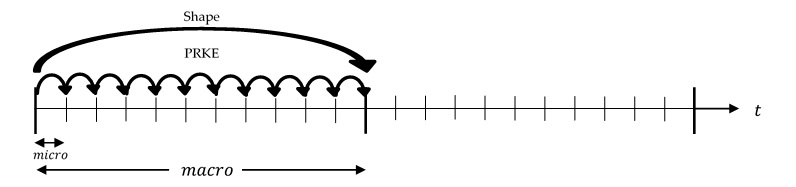
\includegraphics[width=\linewidth]{\FiguresDir/IQS_visualization.jpg}
\caption{IQS method visualization}
\label{fig:iqsviz}
\end{figure}


%%%%%%%%%%%%%%%%%%%%%%%%%%%%%%%%%%%%%%%%%%%%%%%%
\subsection{Iterative Solution Techniques}
\label{sect:iter}
%%%%%%%%%%%%%%%%%%%%%%%%%%%%%%%%%%%%%%%%%%%%%%%%

As we noted in \sct{sect:theory}, shape-PRKE equations are a nonlinear system and thus may be solved in a iterative manner.  Each macro time step can be iterated so the best shape is used to compute power at the micro time steps. Sissaoui et al. from \cite{Sissaoui_1995}, Koclas et al. from \cite{Koclas_1996}, Devooght et al. from \cite{Devooght_1984}, and Monier from \cite{Monier_diss} all use iterative techniques for their quasi-static simulations.  They all undergo a similar process:
\begin{itemize}
\item[\textit{Step 1:}] Compute the PRKE parameters at the end of the macro step using the last computed shape
\item[\textit{Step 2:}] Linearly interpolate the computed PRKE parameters over the macro step
\item[\textit{Step 3:}] Solve the PRKE on micro steps over the entire macro step
\item[\textit{Step 4:}] Solve the shape equation on the macro step using the computed values of $p$ and $dp/dt$.
\item[\textit{Step 5:}] Check if the shape solution has converged:
	\begin{itemize}
	\item \textit{No:} Repeat the same macro time step
	\item \textit{Yes:} Move on to the next macro time step
	\end{itemize}
\end{itemize}

The major difference between the methods of these authors is the convergence criteria used.  Sissaoui and Koclas \cite{Sissaoui_1995, Koclas_1996} use fixed point iteration where the criteria is the simply the normalized difference between the last two computed shapes.  Monier in \cite{Monier_diss} also does fixed point iterations with the same criteria, except the solution is scaled by $\frac{\sum_{g=1}^G\left(\phi^{*g},\frac{1}{v^g}\varphi^g(t_{n})\right)}{\sum_{g=1}^G\left(\phi^{*g},\frac{1}{v^g}\varphi^g(t_{n+1})\right)}$ after each iteration.  Devooght in \cite{Devooght_1984} does a Newton-SOR iteration where the residual of the shape function evaluation is the convergence criteria and next iteration's solution is computed using Newton-Raphson method.\\

These techniques are by no means an exhaustive list of the possible iteration techniques for IQS. Dulla et al. in \cite{Dulla2008} does an in depth analysis of the fixed point iteration technique most similar to Sissaoui and Koclas, involving convergence rates and solution results.  However, no comprehensive analysis of iteration techniques exists, comparing both Newton and fixed-point convergence rates.


%%%%%%%%%%%%%%%%%%%%%%%%%%%%%%%%%%%%%%%%%%%%%%%%
\subsection{Predictor-Corrector version of IQS (IQS P-C)}
\label{sect:pc}
%%%%%%%%%%%%%%%%%%%%%%%%%%%%%%%%%%%%%%%%%%%%%%%%

The Predictor-Corrector (P-C) version of IQS factorizes the flux and derives the PRKE the same way as the standard version, but the solution of the coupled system of equations is different.  In the IQS P-C version, the flux equations (not the shape equations) are solved (represented by Equations~\ref{eq:flux}~and~\ref{eq:precursor}) in order to obtain a predicted flux solution. This predicted flux is then converted to a shape by rescaling it as follows:
\be
\varphi^g_{n+1} = \underbrace{\phi^g_{n+1}}_{\text{predicted}} \frac{K_0}{K_{n+1}}
\label{eq:rescale}
\ee
where the scaling factors are given by
\be
K_{n+1} =\sum_{g=1}^G\left(\phi^{*g},\frac{1}{v^g}\phi^g_{n+1}\right)
\ee
\be
K_{0} =\sum_{g=1}^G\left(\phi^{*g},\frac{1}{v^g}\varphi^g_{n+1}\right)=\sum_{g=1}^G\left(\phi^{*g},\frac{1}{v^g}\phi^g_{0} \,.\right)
\ee

The PRKE parameters are then computed with this shape using Equations~\ref{eq:rmb}~-~\ref{eq:l} and interpolated over the macro step, then the PRKE ODE system is solved on the micro time scale.  With the newly computed amplitude, the shape is rescaled into a flux and the final corrected flux is given by:
\be
\underbrace{\phi^g_{n+1}}_{\text{corrected}} = p_{n+1} \times \varphi^g_{n+1} \,.
\ee

The advantage to the predictor-corrector method is there is no iteration necessary for this method and, in turn, is much simpler and faster than the standard IQS.  Ikeda et al. in \cite{Ikeda_2001} and Goluoglu et al. in \cite{Goluoglu_2001} both use IQS P-C for complex, three-dimensional problems.  Their results prove IQS P-C to be impressively effective, despite the de-coupling of the system.  Dulla et al. in \cite{Dulla2008} also describes an in depth comparison of IQS P-C with traditional IQS.


%%%%%%%%%%%%%%%%%%%%%%%%%%%%%%%%%%%%%%%%%%%%%%%%
%%%%%%%%%%%%%%%%%%%%%%%%%%%%%%%%%%%%%%%%%%%%%%%%
\section{Proposed Research}
\label{sect:research}
%%%%%%%%%%%%%%%%%%%%%%%%%%%%%%%%%%%%%%%%%%%%%%%%
%%%%%%%%%%%%%%%%%%%%%%%%%%%%%%%%%%%%%%%%%%%%%%%%

The proposed research intends to continue the investigation and development of the improved quasi-static method.  

%%%%%%%%%%%%%%%%%%%%%%%%%%%%%%%%%%%%%%%%%%%%%%%%
\subsection{Investigation of Iteration Convergence}
\label{sect:inv_iter}
%%%%%%%%%%%%%%%%%%%%%%%%%%%%%%%%%%%%%%%%%%%%%%%%

\sct{sect:iter} describes several iterative techniques employed for IQS, with different convergence criteria and solution scaling.  A new convergence criteria, not previously attempted, can be applied.  This criteria involves checking that the uniqueness criteria described in \sct{sect:theory} is preserved.  The error of a certain iteration is described by \eqt{eq:eiqs}.  Where $\varphi^{g,n}$ corresponds to the solution at the most recent time step and $\varphi^{g,0}$ corresponds to the initial solution.  This technique is intended to ensure that the solution retains the purity of the analytical derivation.

\be
Error_{IQS}=\left|\frac{\sum_{g=1}^G\left(\phi^{*g},\frac{1}{v^g}\varphi^{g,n}\right)}{\sum_{g=1}^G\left(\phi^{*g},\frac{1}{v^g}\varphi^{g,0}\right)}-1\right|
\label{eq:eiqs}
\ee


This research intends to do investigate the performance of the previously implemented iterative techniques and compare them to this newly implemented technique.

%%%%%%%%%%%%%%%%%%%%%%%%%%%%%%%%%%%%%%%%%%%%%%%%
\subsection{Investigation of Various Time Discretization Schemes}
%%%%%%%%%%%%%%%%%%%%%%%%%%%%%%%%%%%%%%%%%%%%%%%%

A vital part of the verification and validation for IQS is analyzing error convergence.  Since any time discretization scheme is capable of being applied to the shape equation of IQS, it is important to investigate IQS's performance to a variety of these schemes.  There is lack of literature that applies IQS to schemes other than implicit Euler; higher order schemes are never rigorously tested.  This research intends to apply a variety of schemes, including implicit Euler, Crank-Nicholson, backward difference formula (BDF), and diagonally implicit Runge-Kutta (DIRK), to test stability and error convergence.  

%%%%%%%%%%%%%%%%%%%%%%%%%%%%%%%%%%%%%%%%%%%%%%%%
\subsection{Application of Time Adaptation}
%%%%%%%%%%%%%%%%%%%%%%%%%%%%%%%%%%%%%%%%%%%%%%%%

IQS aims at reducing the time discretization error in the flux solution by splitting the flux into an amplitude (that is highly resolved with at a micro time scale) and a shape (whose time-dependence is weaker than that of the flux itself). Thus, by construction, the IQS approach may employ larger time-step sizes for comparable temporal error. Further enhancements can be gained by using time adaptation (or time step control) in order to increase or reduce the macro time step size for the shape evaluation, depending on error estimates. A step-doubling technique is chosen as the time adaptation technique. The step doubling technique involves estimating the local error for a certain time step by taking the difference between a solution with one full step ($\varphi^g_{\Delta t}$) and a solution with two half steps ($\varphi^g_{\Delta t/2}$). Note: $\varphi$ is changed to $\phi$ for implicit discretization and IQS P-C. \\

The relative error is computed as follows:
\be
e_n = \frac{\norm{\sum_{g=1}^G\varphi^g_{\Delta t/2} - \sum_{g=1}^G\varphi^g_{\Delta t}}}{\text{max}\left(\norm{\sum_{g=1}^G\varphi^g_{\Delta t/2}},\norm{\sum_{g=1}^G\varphi^g_{\Delta t}}\right)}
\label{eq:edt2}
\ee
If the error is smaller than the user-specified tolerance, $e_{tol}$, the time step is accepted. In addition, a new time step size is estimated as follows:
\be
\Delta t_{new} = S \Delta t \left(\frac{e_{tol}}{e_n}\right)^{\frac{1}{1+q}}
\label{eq:dt2}
\ee
Where $q$ is the convergence order of the time integration scheme being used and $S\simeq 0.8$ is a safety factor. If the error is larger than the user-specified tolerance, the time step is rejected. A new time step size is estimated using  \eqt{eq:edt2} as well. \\

To investigate IQS's performance with step-doubling time adaptation, the adaptation will be applied to implicit discretization method, traditional IQS, and IQS P-C.  Each of these methods will be applied to several diffusion problems; the number of time steps taken and the resulting error will be used to compare the methods.

%%%%%%%%%%%%%%%%%%%%%%%%%%%%%%%%%%%%%%%%%%%%%%%%
\subsection{Application of Temperature Feedback}
%%%%%%%%%%%%%%%%%%%%%%%%%%%%%%%%%%%%%%%%%%%%%%%%

IQS is first and foremost a nuclear reactor simulation method.  In nuclear reactors, multiple physics affect the profile of the neutron flux.  The most simple example of mulitphysics reactor simulations is adiabatic heat up with Doppler feedback. The principle of Doppler feedback is that fission in a fuel causes the material to increase temperature and induces a change in the neutronics properties.  The material heat up is described by \eqt{eq:temp}; where $\rho$ is the material density, $c_p$ is the specific heat, $T$ is temperature, and $\kappa_f$ is the energy released per fission \cite{ANL_BPB}. The change in temperature of the material mainly affects the thermal macroscopic absorption cross section described by \eqt{eq:dopp} \cite{ANL_BPB}.

\be
\rho c_p \frac{\partial T(\vec{r},t)}{\partial t} = \kappa_f \sum^G_{g=1}\Sigma_f^g \phi^g(\vec{r},t)
\label{eq:temp}
\ee

\be
\Sigma_a^{thermal}(\vec{r},t) = \Sigma_a^{thermal}(\vec{r},0)\left[1+\gamma\left(\sqrt{T}-\sqrt{T_0}\right)\right]
\label{eq:dopp}
\ee

For IQS, this temperature feedback affects both the shape equation and the reactivity of the PRKE; thus, it is an additional nonlinear component to the already coupled shape-amplitude equations. In foresight to the application of this component, temperature is much more time dependent than the shape, but less so than the amplitude.  Therefore, the evaluation of temperature will have its own time scale.  A possible solution process for a problem with temperature feedback will have time three time scales portrayed in \fig{fig:time}.  The first time scale is the shape solve, the second is the temperature evaluation as well as the computation of PRKE parameters, and the third is the PRKE scale.

\begin{figure}[htpb!]
\centering
\begin{tikzpicture}[scale=2]
%Shape
\draw[] (0,2) -- (6,2) ;
\foreach \x in  {0,6}
\draw[shift={(\x,2)},color=black] (0pt,6pt) -- (0pt,-6pt);
\draw[shift={(0,2)},color=black] (0pt,0pt) -- (0pt,-6pt) node[below] {$t_n$};
\draw[shift={(6,2)},color=black] (0pt,0pt) -- (0pt,-6pt) node[below] {$t_{n+1}$};
\node(shape) at (-.25,2) {$\varphi:$};

%Temp/Params
\draw[] (0,1) -- (6,1) ;
\foreach \x in  {0,6}
\draw[shift={(\x,1)},color=black] (0pt,6pt) -- (0pt,-6pt);
\foreach \x in  {2,4}
\draw[shift={(\x,1)},color=black] (0pt,4pt) -- (0pt,-4pt);
\draw[shift={(0,1)},color=black] (0pt,0pt) -- (0pt,-6pt) node[below] {$t_n$};
\draw[shift={(6,1)},color=black] (0pt,0pt) -- (0pt,-6pt) node[below] {$t_{n+1}$};
\node(temp) at (-.75,1) {$T \rightarrow \rho, \bar{\beta}, \bar{\lambda}, \Lambda$:};

% PRKE
\draw[] (0,0) -- (6,0) ;
\foreach \x in  {0,6}
\draw[shift={(\x,0)},color=black] (0pt,6pt) -- (0pt,-6pt);
\foreach \x in  {0,2,4,6}
\draw[shift={(\x,0)},color=black] (0pt,4pt) -- (0pt,-4pt);
\foreach \x in  {0,0.2,0.4,0.6,0.8,1,1.2,1.4,1.6,1.8,2,2.2,2.4,2.6,2.8,3,3.2,3.4,3.6,3.8,4,4.2,4.4,4.6,4.8,5,5.2,5.4,5.6,5.8,6}
\draw[shift={(\x,0)},color=black] (0pt,2pt) -- (0pt,-2pt);
\draw[shift={(0,0)},color=black] (0pt,0pt) -- (0pt,-6pt) node[below] {$t_n$};
\draw[shift={(6,0)},color=black] (0pt,0pt) -- (0pt,-6pt) node[below] {$t_{n+1}$};
\node(prke) at (-.5,0) {$p, \frac{dp}{dt}:$};

\draw (0,0) edge[out=45,in=135,->,thick] node[above,sloped] {Step 2} (2,0);
\draw (2,0) edge[out=45,in=135,->,thick] node[above,sloped] {Step 4} (4,0);
\draw (4,0) edge[out=45,in=135,->,thick] node[above,sloped] {Step 6} (6,0);
\draw (0,1) edge[out=45,in=135,->,thick] node[above,sloped] {Step 1} (2,1);
\draw (2,1) edge[out=45,in=135,->,thick] node[above,sloped] {Step 3} (4,1);
\draw (4,1) edge[out=45,in=135,->,thick] node[above,sloped] {Step 5} (6,1);
\draw (0,2) edge[out=15,in=165,->,thick] node[above,sloped] {Step 7} (6,2);

\draw (0,2) edge[out=-135,in=135,->,thick] node[below,sloped] {$\varphi$} (0,1);
\draw (2,1) edge[out=-135,in=135,->,thick] node[below,sloped] {$\rho$} (2,0);
\draw (2,0) edge[out=45,in=-45,->,thick] node[below,sloped] {$p$} (2,1);
\draw (4,1) edge[out=-135,in=135,->,thick] node[below,sloped] {$\rho$} (4,0);
\draw (4,0) edge[out=45,in=-45,->,thick] node[below,sloped] {$p$} (4,1);
\draw (6,1) edge[out=-135,in=135,->,thick] node[below,sloped] {$\rho$} (6,0);
\draw (6,0) edge[out=45,in=0,->,thick] node[below,sloped] {$p, \frac{dp}{dt}$} (6,2);

\end{tikzpicture}
\caption{Time scales and process of IQS with temperature feedback}
\label{fig:time}
\end{figure}

The couplings between temperature, amplitude, and shape are all nonlinear, so iteration processes are need for each time scale.  The amplitude and temperature need to be iterated on the middle time scale until convergence on each temperature step.  Then another iterative process needs to occur in the shape time scale scale on all three variables.

%%%%%%%%%%%%%%%%%%%%%%%%%%%%%%%%%%%%%%%%%%%%%%%%
\subsection{Implementation into Rattlesnake/MOOSE Framework}
%%%%%%%%%%%%%%%%%%%%%%%%%%%%%%%%%%%%%%%%%%%%%%%%

A one-dimensional, single group FEM prototype will be created for IQS in order to test validation for simple problems. However, testing complex, real-world problems is most easily performed by implementing IQS in a FEM framework.  The Rattlesnake radiation transport framework is a excellent option for performing these problems.  Rattlesnake already contains a neutron diffusion method for continuous-FEM equivalent to the implicit discretization method.  Additionally, Rattlesnake is well documented and well organized, so implementing IQS may be relatively straightforward. With this implementation, benchmark testing such as 16-A1 \cite{ANL_BPB}, TWIGL, LRA, C5G7-2D, etc. can be performed, as well as a full core simulation of the TREAT reactor.

%%%%%%%%%%%%%%%%%%%%%%%%%%%%%%%%%%%%%%%%%%%%%%%%
%%%%%%%%%%%%%%%%%%%%%%%%%%%%%%%%%%%%%%%%%%%%%%%%
\newpage
\section{Preliminary Results}
\label{sect:results}
%%%%%%%%%%%%%%%%%%%%%%%%%%%%%%%%%%%%%%%%%%%%%%%%
%%%%%%%%%%%%%%%%%%%%%%%%%%%%%%%%%%%%%%%%%%%%%%%%

This section describes preliminary results of an example that tests an IQS implementation and shows its effectiveness on computation speed and accuracy.  The example is very simple and computes quickly, it entails a one dimensional, homogeneous 400 cm slab with a heterogenous perturbation in absorption cross section.  \fig{fig:slab} shows how the regions of the slab are divided and \tbl{tab:1Dmat} shows the initial material properties.  Regions 2, 3, and 4 have slope perturbations at different points in time, \tbl{tab:1Dslope} shows the values of the absorption cross-section in each region at the times of interest.  The values of $\Sigma_a$ between these times of interest are linear interpolations between the given values. \\

\begin{figure}[!htbp]
\begin{center}
\begin{tabular}{| l | l | l | l | l | l | l | l | l | l | l | l | l | l | l | l | l | l | l | l |}
\hline \hline \hline
  &   &   &   &   &   &    &    &   &   &   &   &   &   &   &   &   &   &   &   \\
1 & 1 & 1 & 1 & 2 & 3 & 1 & 1 & 1 & 1 & 1 & 1 & 1 & 1 & 4 & 4 & 1 & 1 & 1 & 1 \\
  &   &   &   &   &   &    &    &   &   &   &   &   &   &   &   &   &   &   &   \\
\hline \hline \hline
\end{tabular}
\caption{1-D slab region identification}
\label{fig:slab}
\end{center}
\end{figure}

\begin{table}[!htbp]
\begin{center}
\caption{1-D slab material properties and problem parameters}
\label{tab:1Dmat}
\begin{tabular}{llllll}
\hline
$D (cm)$ & $\Sigma_a (cm^{-1})$ & $\nu \Sigma_f (cm^{-1})$ & $v (cm/s)$ & $\beta$ & $\lambda (s^{-1})$ \\
\hline
1.0 & 1.1 & 1.1 & 1,000 & 0.006 & 0.1 \\

\hline
\end{tabular}
\end{center}
\end{table}

\begin{table}[!htbp]
\begin{center}
\caption{1-D slab absorption cross-section at times of interest}
\label{tab:1Dslope}
\begin{tabular}{llllllll}
\hline
Region & Material Property & 0.0 s & 0.1 s & 0.6 s & 1.0 s & 1.7 s \\
\hline
2 & $\Sigma_{a} (cm^{-1})$ & 1.1 & 1.1 & 1.095 & 1.095 & 1.095 \\
3 & $\Sigma_{a} (cm^{-1})$ & 1.1 & 1.1 & 1.09 & 1.09 & 1.1 \\
4 & $\Sigma_{a} (cm^{-1})$ & 1.1 & 1.1 & 1.105 & 1.105 & 1.105 \\
\hline
\end{tabular}
\end{center}
\end{table}



\fig{fig:power} shows the power at each macro time step as compared to the traditional brute force (full flux implicit discretization) method.  The strong correlation between the two curves shows that IQS is consistent with a proven method for a highly transient example. \fig{fig:conv} shows the error convergence for implicit discretization and IQS methods.  This plot shows that IQS has consistent convergence slope for first and second order time schemes and that IQS has a better error constant for the convergence.  \tbl{tab:1Ddt2} shows the results for time adaptation.  These results show that traditional IQS does not perform well with step doubling time adaptation and IQS P-C performs moderately better than implicit discretization.  The IQS performance in this example are not exceptional because it is not an easy problem.  As seen in \fig{fig:1D_shape}, the shape undergoes significant change through the transient, which requires many shape evaluations to retain accuracy.

\begin{figure}[!htbp]
\centering
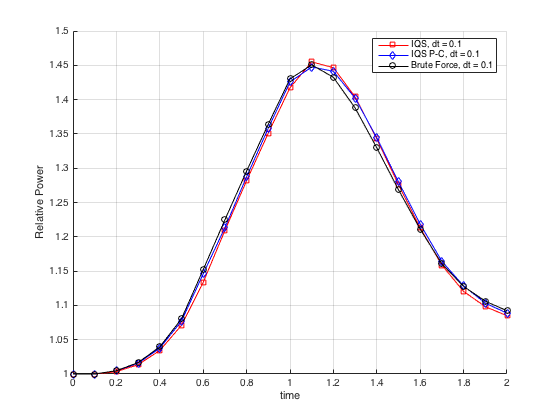
\includegraphics[width=0.49\textwidth]{\FiguresDir/1D_het_power_plot.png}
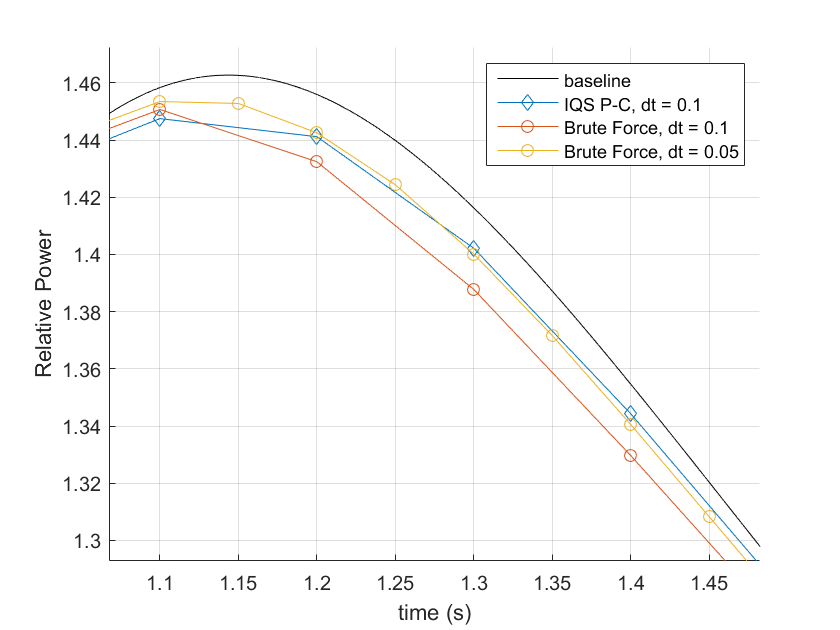
\includegraphics[width=0.5\textwidth]{\FiguresDir/1D_het_power_plot2.png}
\caption{Power level of 1D example}
\label{fig:power}
\end{figure}

\begin{figure}[!htbp]
\centering
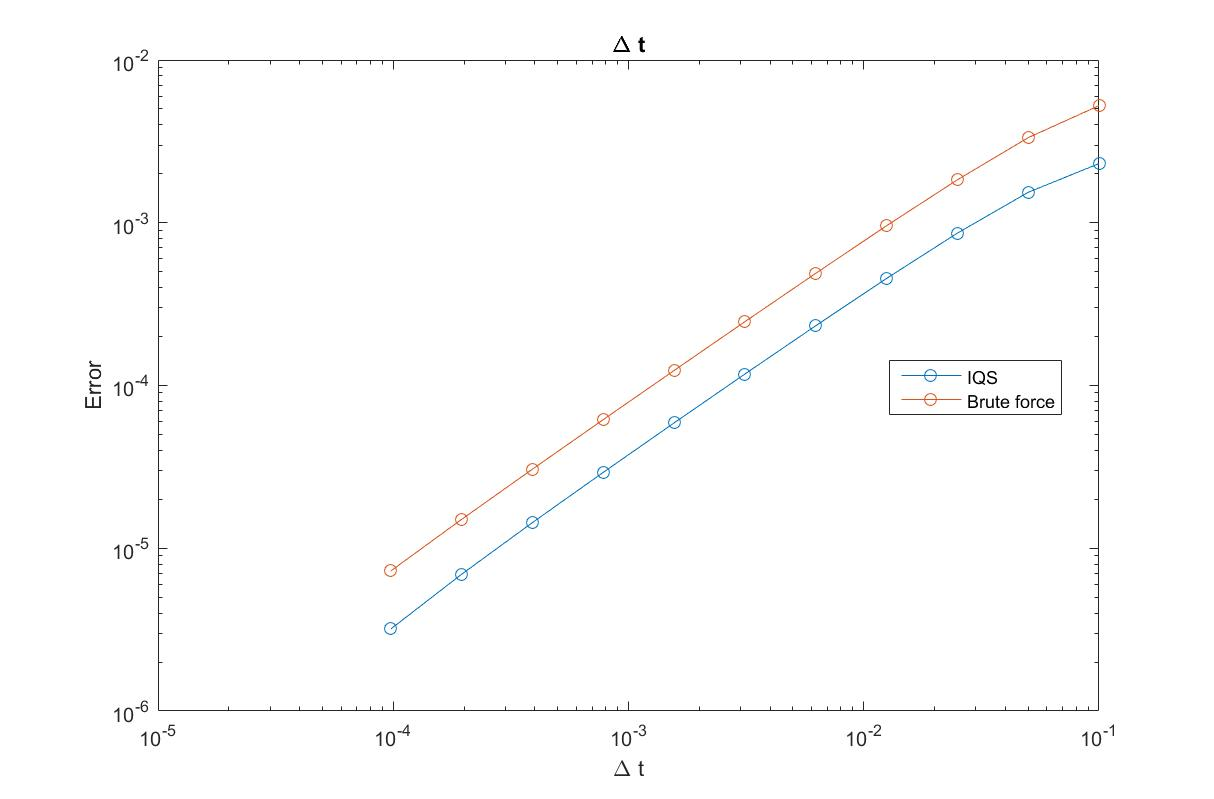
\includegraphics[width=5in]{\FiguresDir/1D_het_convergence.jpg}
\caption{Error convergence comparison of 1D example}
\label{fig:conv}
\end{figure}

\begin{table}[!htbp]
\begin{center}
\caption{1-D slab step doubling results}
\label{tab:1Ddt2}
\resizebox{\textwidth}{!}{
\begin{tabular}{|l|l|l|l|l|l|l|l|l|l|l|}
\hline
  &  & \multicolumn{3}{|c|}{Implicit Discretization} & \multicolumn{3}{|c|}{IQS} & \multicolumn{3}{|c|}{IQS P-C} \\
\hline
Test & $e_{tol}$ & Error & Steps & Solves & Error & Steps & Solves & Error & Steps & Solves \\
\hline
1 &	0.05 	&	0.021596 &	10  &	32	 &	0.10084 &	12	  &	175		&	0.028019 &	10	&	33 \\
2 &	0.01 	&	0.032864 &	21  &	80	 &	0.08030 &	41	  &	850	 	&	0.044721 &	20	&	74 \\
3 &	0.005 	&	0.053159 &	27  &	96	 &	0.01215 &	115	  &	2220 	&	0.052095 &	25	&	96 \\
4 & 0.001 	&	0.056546 &	56  &	188	 &	0.03242 &	848	  &	12511 	&	0.061274 &	50	&	162 \\
5 &	0.0005 	&	0.062882 &	77  &	245	 &	0.03491 &	1718  &	25841 	&	0.061240 &	69	&	225 \\
6 &	0.0001 	&	0.060089 &	177 &	537	 &	0.03554 &	8702  &	129985 	&	0.060824 &	159	&	480 \\
7 &	5.0e-05	&	0.059513 &	252 &	767	 &	0.03622 &	17282 &	256463 	&	0.061078 &	224	&	680 \\
8 &	1.0e-05	&	0.061063 &	561 &	1691 &	0.03142 &	79988 &	1104227 &	0.061901 &	501	&	1509 \\
\hline
\end{tabular}}
\end{center}
\end{table}

\begin{figure}[!htbp]
\begin{center}
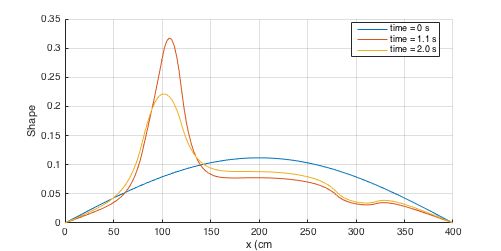
\includegraphics[width=\linewidth]{\FiguresDir/1D_shape.png}
\caption{Flux profile of 1D slab at various times}
\label{fig:1D_shape}
\end{center}
\end{figure}

%%%%%%%%%%%%%%%%%%%%%%%%%%%%%%%%%%%%%%%%%%%%%%%%
%%%%%%%%%%%%%%%%%%%%%%%%%%%%%%%%%%%%%%%%%%%%%%%%
\newpage
\section{Goals of Proposed Research}
\label{sect:goals}
%%%%%%%%%%%%%%%%%%%%%%%%%%%%%%%%%%%%%%%%%%%%%%%%
%%%%%%%%%%%%%%%%%%%%%%%%%%%%%%%%%%%%%%%%%%%%%%%%

\begin{enumerate}[topsep=0pt,itemsep=-1ex,partopsep=1ex,parsep=1ex]
\item Investigate iteration convergence for previously implemented iterative schemes and newly conceived one described in \sct{sect:inv_iter}.
\item Verify IQS method with several low and high order time discretization schemes.
\item Implement step doubling time adaptation with IQS and analyze its performance compared to implicit discretization of the flux equations.
\item Apply temperature feedback with IQS and analyze its performance with multiphysics benchmarks.
\item Implement IQS into the Rattlesnake framework at INL.
\item Perform testing with IQS to benchmarks including TWIGL, LRA, and LMW.
\end{enumerate}

%%%%%%%%%%%%%%%%%%%%%%%%%%%%%%%%%%%%%%%%%%%%%%%%
\subsection{Possible Extensions}
%%%%%%%%%%%%%%%%%%%%%%%%%%%%%%%%%%%%%%%%%%%%%%%%

Some extensions, beyond the proposed scope of this research, have been identified as follows:

\begin{enumerate}[topsep=0pt,itemsep=-1ex,partopsep=1ex,parsep=1ex]
\item Perform a full core simulation of TREAT with IQS.
\item Investigate other multiphysics coupling with IQS including structural mechanics and thermal hydraulics.
\item Investigate IQS application to self-adjoint angular flux S$_\text{N}$ (SAAF-SN).
\end{enumerate}

%%%%%%%%%%%%%%%%%%%%%%%%%%%%%%%%%%%%%%%%%%%%%%%%%%%%%%%%%%%%%%%%%%%%%%%%%%%%%
%%%%%%%%%%%%%%%%%%%%%%%%%%%%%%%%%%%%%%%%%%%%%%%%%%%%%%%%%%%%%%%%%%%%%%%%%%%%%
\newpage
\bibliographystyle{abbrvnat}
\bibliography{references_IQS}

%%%%%%%%%%%%%%%%%%%%%%%%%%%%%%%%%%%%%%%%%%%%%%%%%%%%%%%%%%%%%%%%%%%%%%%%%%%%%%%%

\end{document}